\documentclass{article}
\usepackage{indentfirst}
\usepackage[utf8]{inputenc}
\usepackage[margin=0.5in]{geometry}
\usepackage{graphicx}

\begin{document}

\title{Glossario di SWE}
\author{M9k}
\maketitle

%\section{TEXT}
%\subsection{TEXT}
%\subsubsection{TEXT}
%\paragraph{TEXT}
%\subparagraph{Subparagraph}Subparagraph text.\vspace{2mm}

\section{Introduzione}
	
	\subsection{Termini base}
		\textbf{Progetto}\\
		Insieme di attività e compiti\\
		-per raggiungere obbiettivi con specifiche fissate\\
		-data di inizio e di fine fissate\\
		-risorse limitate (es: persone, tempo, fondi, strumenti)\\
		-consuma risorse svolgendosi\\
			
		\textbf{Processo}\\
		\textit{Insieme di attività correlate} e \textit{coese} che trasformano ingressi (bisogni) in uscite (prodotti) secondo regole date, consumando risorse nel farlo\\
		
		\textbf{Attività}\\
		Cosa da fare per il raggiungimento degli obbiettivi, composta da più compiti\\
		
		\textbf{Compito}\\
		Cosa che una persona deve fare\\

		\textbf{Processi, attività, tasks/compiti}\\
		-Processo: attività correlate che trasformano i bisogni in prodotti, ed: sviluppo, documentazione, qualifica...\\
		-Attività: cosa che voglio fare per poter completare un processo\\
		-Task/compito: cosa che qualcuno deve fare per realizzare l'attività\\
			
		\textbf{Esempi attività e compiti:}\\
		-Pianificazione (\textit{gestione risorse} e \textit{responsabilità})\\
		-Analisi dei requisiti (\textsl{cosa} devo fare)\\
		-Progettazione (\textit{come} farlo)\\
		-Realizzazione (con una \textit{qualità}, \textit{verificando} la correttezza, \textit{validando} i risultati)\\
		
		\textbf{Efficienza}\\
		Produttività, metrica del grado di riduzione degli sprechi\\
		Quantità prodotto realizzato/risorse utilizzate\\
		
		\textbf{Efficacia}\\
		Qualità, metrica del grado di raggiungimento degli obbiettivi interni (del fornitore) o esterni (gradimento del cliente)\\
		
		\textbf{Prodotto SW}\\
		È un insieme di parti, che stanno assieme secondo la loro \textit{configurazione}.\\
		Ogni sistema fatto di parti va gestito con il \textit{controllo di configurazione}.
			
			
			
			
		
		
		
			
	\clearpage
	\subsection{Ingegneria}
		\textbf{Ingegneria}\\
			Applicazioni principi matematici e scientifici a scopo pratico, NON per esplorare nuove possibilità o espandere la scienza\\
			Mai inventare, utilizzare sempre metodi testati e funzionanti\\
			
		\textbf{Best practice}\\
		Miglior modo (way of working) per raggiungere uno scopo, secondo applicazioni passate che hanno dimostrato i risultati\\
		
		\textbf{Pratical ends}\\
		Avere un fine civile e sociale oltre che economico\\
		
	\subsection{Ingegneria del software}
		\textbf{Ingegneria del software}\\
		Disciplina per la realizzazione di \textit{prodotti software} impegnativo e che richiede collaborazione\\
		-in grande e in piccolo (tanto in quantità o poco e specializzato)\\
		-con qualità = \textit{efficacia} = grado di conformità, capacità di raggiungere gli obiettivi\\
		-con costi e tempi contenuti = \textit{efficienza} = capacità di ridurre le risorse e gli sprechi, seguendo la best practice \\
		-tutto lungo il \textit{ciclo di vita}\\
		
		\textbf{Ingegneria del software}\\
		Raccogliere, organizzare e consolidare conoscenza (body of knowledge) necessarie a realizzare progetti SW con massima efficacia e efficenza.\\
		Acquisire, utilizzare e mantenere i best practice.\\
		
		
		\textbf{Ingegneria del software}\\
		Secondo IEEE: Approccio \textit{sistematico}, \textit{disciplinato} e \textit{quantificato} allo sviluppo, uso, manutenzione e ritiro del SW.\\
		Sistematico: metodico e rigoroso, usando una metodologia precisa, per studiare ed evolvere best practice\\
		Disciplinato: regole fissate\\
		Quantificabile: efficienza ed efficacia misurabili.\\
		
		
		\textbf{Tipologie di prodotti software}\\
		-Commessa: forma, contenuto e funzioni definiti dal committente\\
		-Pacchetto: forma, contenuto e funzioni idonei alla replicazione\\
		-Componente: forma, contenuto e funzioni idonei alla composizione\\
		-Servizio: forma, contenuto e funzioni definiti dal problema\\
		
		\textbf{Le 4 P di SWE}\\
		-People (stakeholder e team di sviluppo)\\
		-Product (SW e documentazione)\\
		-Project (Insieme di attività di produzione)\\
		-Process (way of working)\\
		
		\textbf{Ciclo di vita}\\
		Insieme di stati di avanzamento del software fino al ritiro\\
		Un ciclo di vita lungo porta a elevati costi di \textit{manutenzione}\\
		
		\textbf{Manutenzione}\\
		-correttiva: fix dei bug\\
		-adattiva: rifinisco i requisiti\\
		-evolutiva: evoluzione del software secondo i nuovi usi\\
		
		\textbf{Utilità}\\
		\textit{Metrica} riguardante gli utilizzi/utenti di un prodotto nel tempo\\
		
		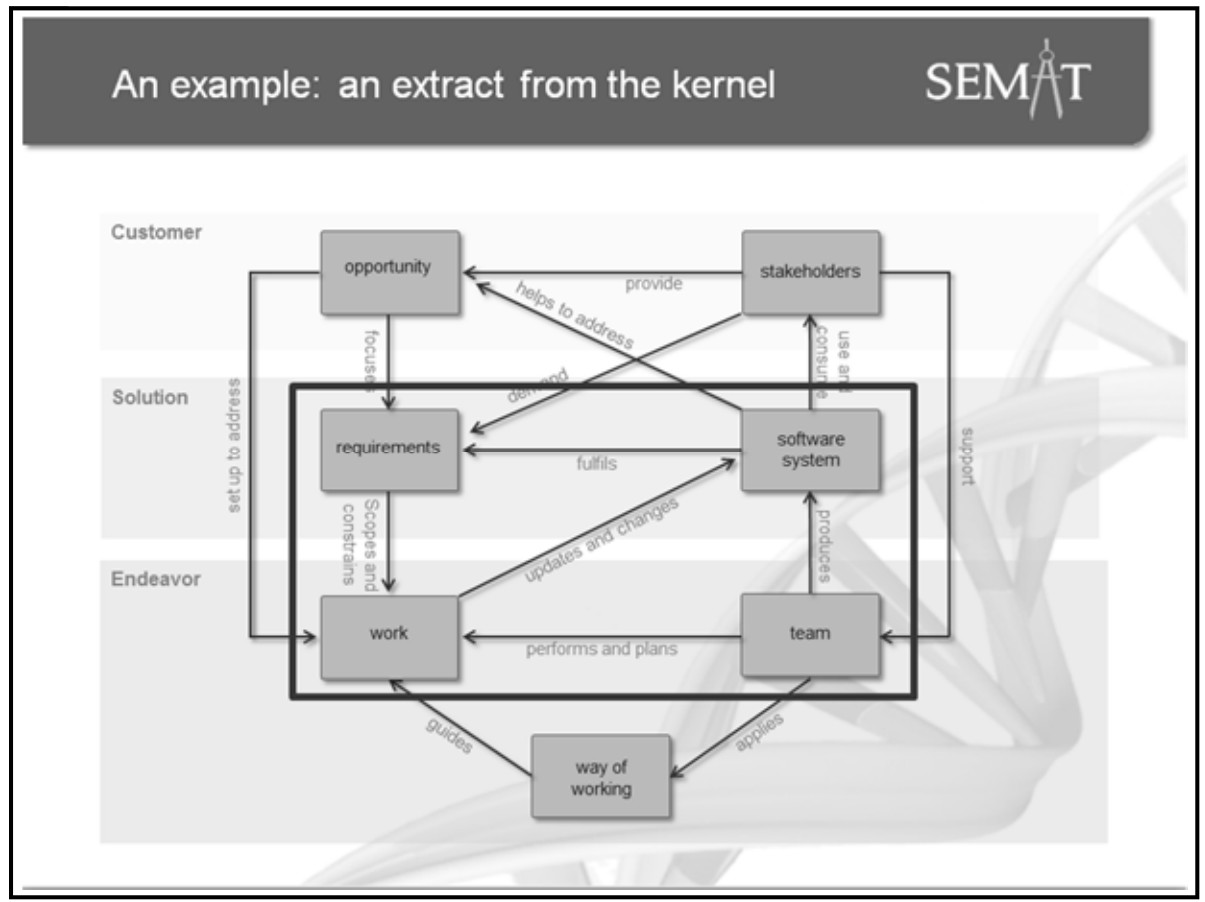
\includegraphics[width=14cm]{semat_org.jpg}\\
		
		
	\clearpage
	\subsection{Processi SW}
		\textbf{Ciclo di vita}\\
		Gli stati che il prodotto assume dal concepimento al ritiro\\
		Serve per valutare costi, tempi, obblighi e rischi PRIMA di svolgere il progetto\\
		Scelta tra più possibili cicli di vita, ognuno con vantaggi e limiti\\
		
		\textbf{Processi di ciclo di vita}\\
		Specificano le attività da svolgere per abilitare corrette transizioni di stato nel ciclo di vita\\
		
		
		\textbf{Modelli di ciclo di vita}\\
		Descrivono come i processi di ciclo di vita si relazionano tra di loro rispetto agli stati\\
		Aiutano a pianificare, organizzare ed eseguire lo svolgimento delle attività\\
		
		
		\textbf{Visione a grafi}\\
		Gli stati sono i nodi (concezione, sviluppo, utilizzo, ritiro, etc), gli archi le attività svolte sul prodotto necessarie per farlo avanzare.\\
		Natura degli stati e pre- e post- condizione determinate da \textit{obblighi} (vincoli contrattuali), \textit{regole} (standard di processo) e \textit{strategie}\\
		
		\subsubsection{Modelli di sviluppo}
			\textbf{Modelli più significativi}\\
			-Sequenziale o a cascata (waterfall)\\
			-Incrementale\\
			-A evoluzioni successive\\
			-A spirale\\
			-Per componenti\\
			-Agile\\
		
			
			\textbf{Iterazionale}\\
			Procedere per raffinamento o rivisitazioni (pittura)\\
			
			\textbf{Incremento}\\
			Procedere per aggiunta a un impianto base (scultura)\\
			
			\textbf{Prototipo}\\
			Per provare e scegliere, usa e getta oppure avere avanzamento incrementale (baseline)\\
			
			\textbf{Riuso}\\
			-Occasionale: copia-incolla, basso costo, scarso impatto\\
			-Sistematico: per progetto/prodotto/azienda, maggior costo, maggior impatto\\
			
			
			\textbf{Standard di processo}\\
			Aiuta a raggiungere l'economicità, riferimento a ISO/IEC 12207:1995\\
			Nascono per \textit{iniziativa del committente} per facilitare \textit{controllo}, \textit{collaudo} e \textit{accettazione}\\
			
			\textbf{Standard come modello di azione}\\
			Definizione e imposizione di \textit{procedure}, definizione e proposizione di \textit{processi da specializzare}\\
			
			\textbf{Standard come modello di valutazione}\\
			Modelli più generali, copre più contesti, per identificare best practice\\
		
			\textbf{ISO/IEC 12207:1995}\\
			Più diffuso, ad alto livello\\
			Identifica i processi di ciclo di vita del SW\\
			Struttura modulare che richiede specializzazione\\
			Specifica le responsabilità sui processi e i prodotti\\
			
			\textbf{Processi primari}\\
			Necessari per l'esistenza di un progetto\\
			-Acquisizione (gestione dei sotto-fornitori)\\
			-Fornitura (gestione rapporti con il cliente)\\
			-Sviluppo\\
			-Gestione operativa (utilizzo, erogazione, installazione)\\
			-Manutenzione (correzione, adattamento, evoluzione)\\
			
			\textbf{Processi di supporto}\\
			-Documentazione\\
			-Accertamento qualità\\
			-Gestione delle versioni e delle configurazioni\\
			-Qualifica: verifica + validazione\\
			-Revisioni congiunte con il cliente\\
			-Verifiche ispettive interne\\
			-Risoluzione dei problemi (gestione dei cambiamenti)\\
			
			\textbf{Processi organizzativi}\\
			-Gestione dei processi\\
			-Gestione delle infrastrutture\\
			-Miglioramento del processo\\
			-Formazione personale\\
			
			
			\textbf{SONO ARRIVATO A SLIDE 22/36}\\
			
			
			
			
			
			
			
			
			
	
\end{document}
